% File for libamtrack manual
% Copyright 2006, 2010 Steffen Greilich / the libamtrack team
% This file is part of the libAmTrack project (libamtrack.dkfz.org).

\chapter{Electron range relation}
\label{chap:ERs}

The submodels of electron-range relation determining the width of the particle tracks (Tab. \ref{tbl:ERs} and Fig. \ref{fig:ERs}) -- their differences can be up to two orders of magnitude at the upper end of the range of clinically used energies.


\begin{table}
\label{tbl:ERs}
\begin{tabular}{m{0.25\textwidth}p{0.60\textwidth}m{0.15\textwidth}}

\hline
\textbf{Name} & \textbf{Expression} & \textbf{Reference} \\
\hline

\begin{center}Butts and Katz\end{center}&
$r_{max}/\text{(g$\cdot$cm$^{-2}$)}=10^{-6}\cdot w/\text{keV} \text{   , with   } w/\text{keV}=2\cdot m_e\cdot ((\frac{E}{E_0})^2+2(\frac{E}{E_0})$
&\cite{Butts_and_Katz_1967}\\

\begin{center}Walig\'orski\end{center}&
$r_{max}/\text{(g$\cdot$cm$^{-2}$)}=6\cdot 10^{-6}\cdot (w/\text{keV})^\alpha \text{   , with   } \alpha=1.079(w<1\text{ keV) or } 1.667\text{ (otherwise)}$
&\cite{Waligorski_et_al_1986}\\

\begin{center}Geiss\end{center}&
$r_{max}/\text{cm}=4\cdot 10^{-5}\cdot (E/\text{MeV})^{1.5}\cdot \frac{\rho_{material}}{\rho_{water}}$
&\cite{Geiss_1998}\\

\begin{center}Scholz\end{center}&
$r_{max}/\text{$\mu$m}=0.05\cdot 10^{-5}\cdot (E/\text{MeV})^{1.7}\cdot \frac{\rho_{material}}{\rho_{water}}$
&\cite{Scholz_2001}\\

\hline
\end{tabular}
\caption{ERs implemented in \la{}.}
\end{table}


\begin{figure*}
	\centering
		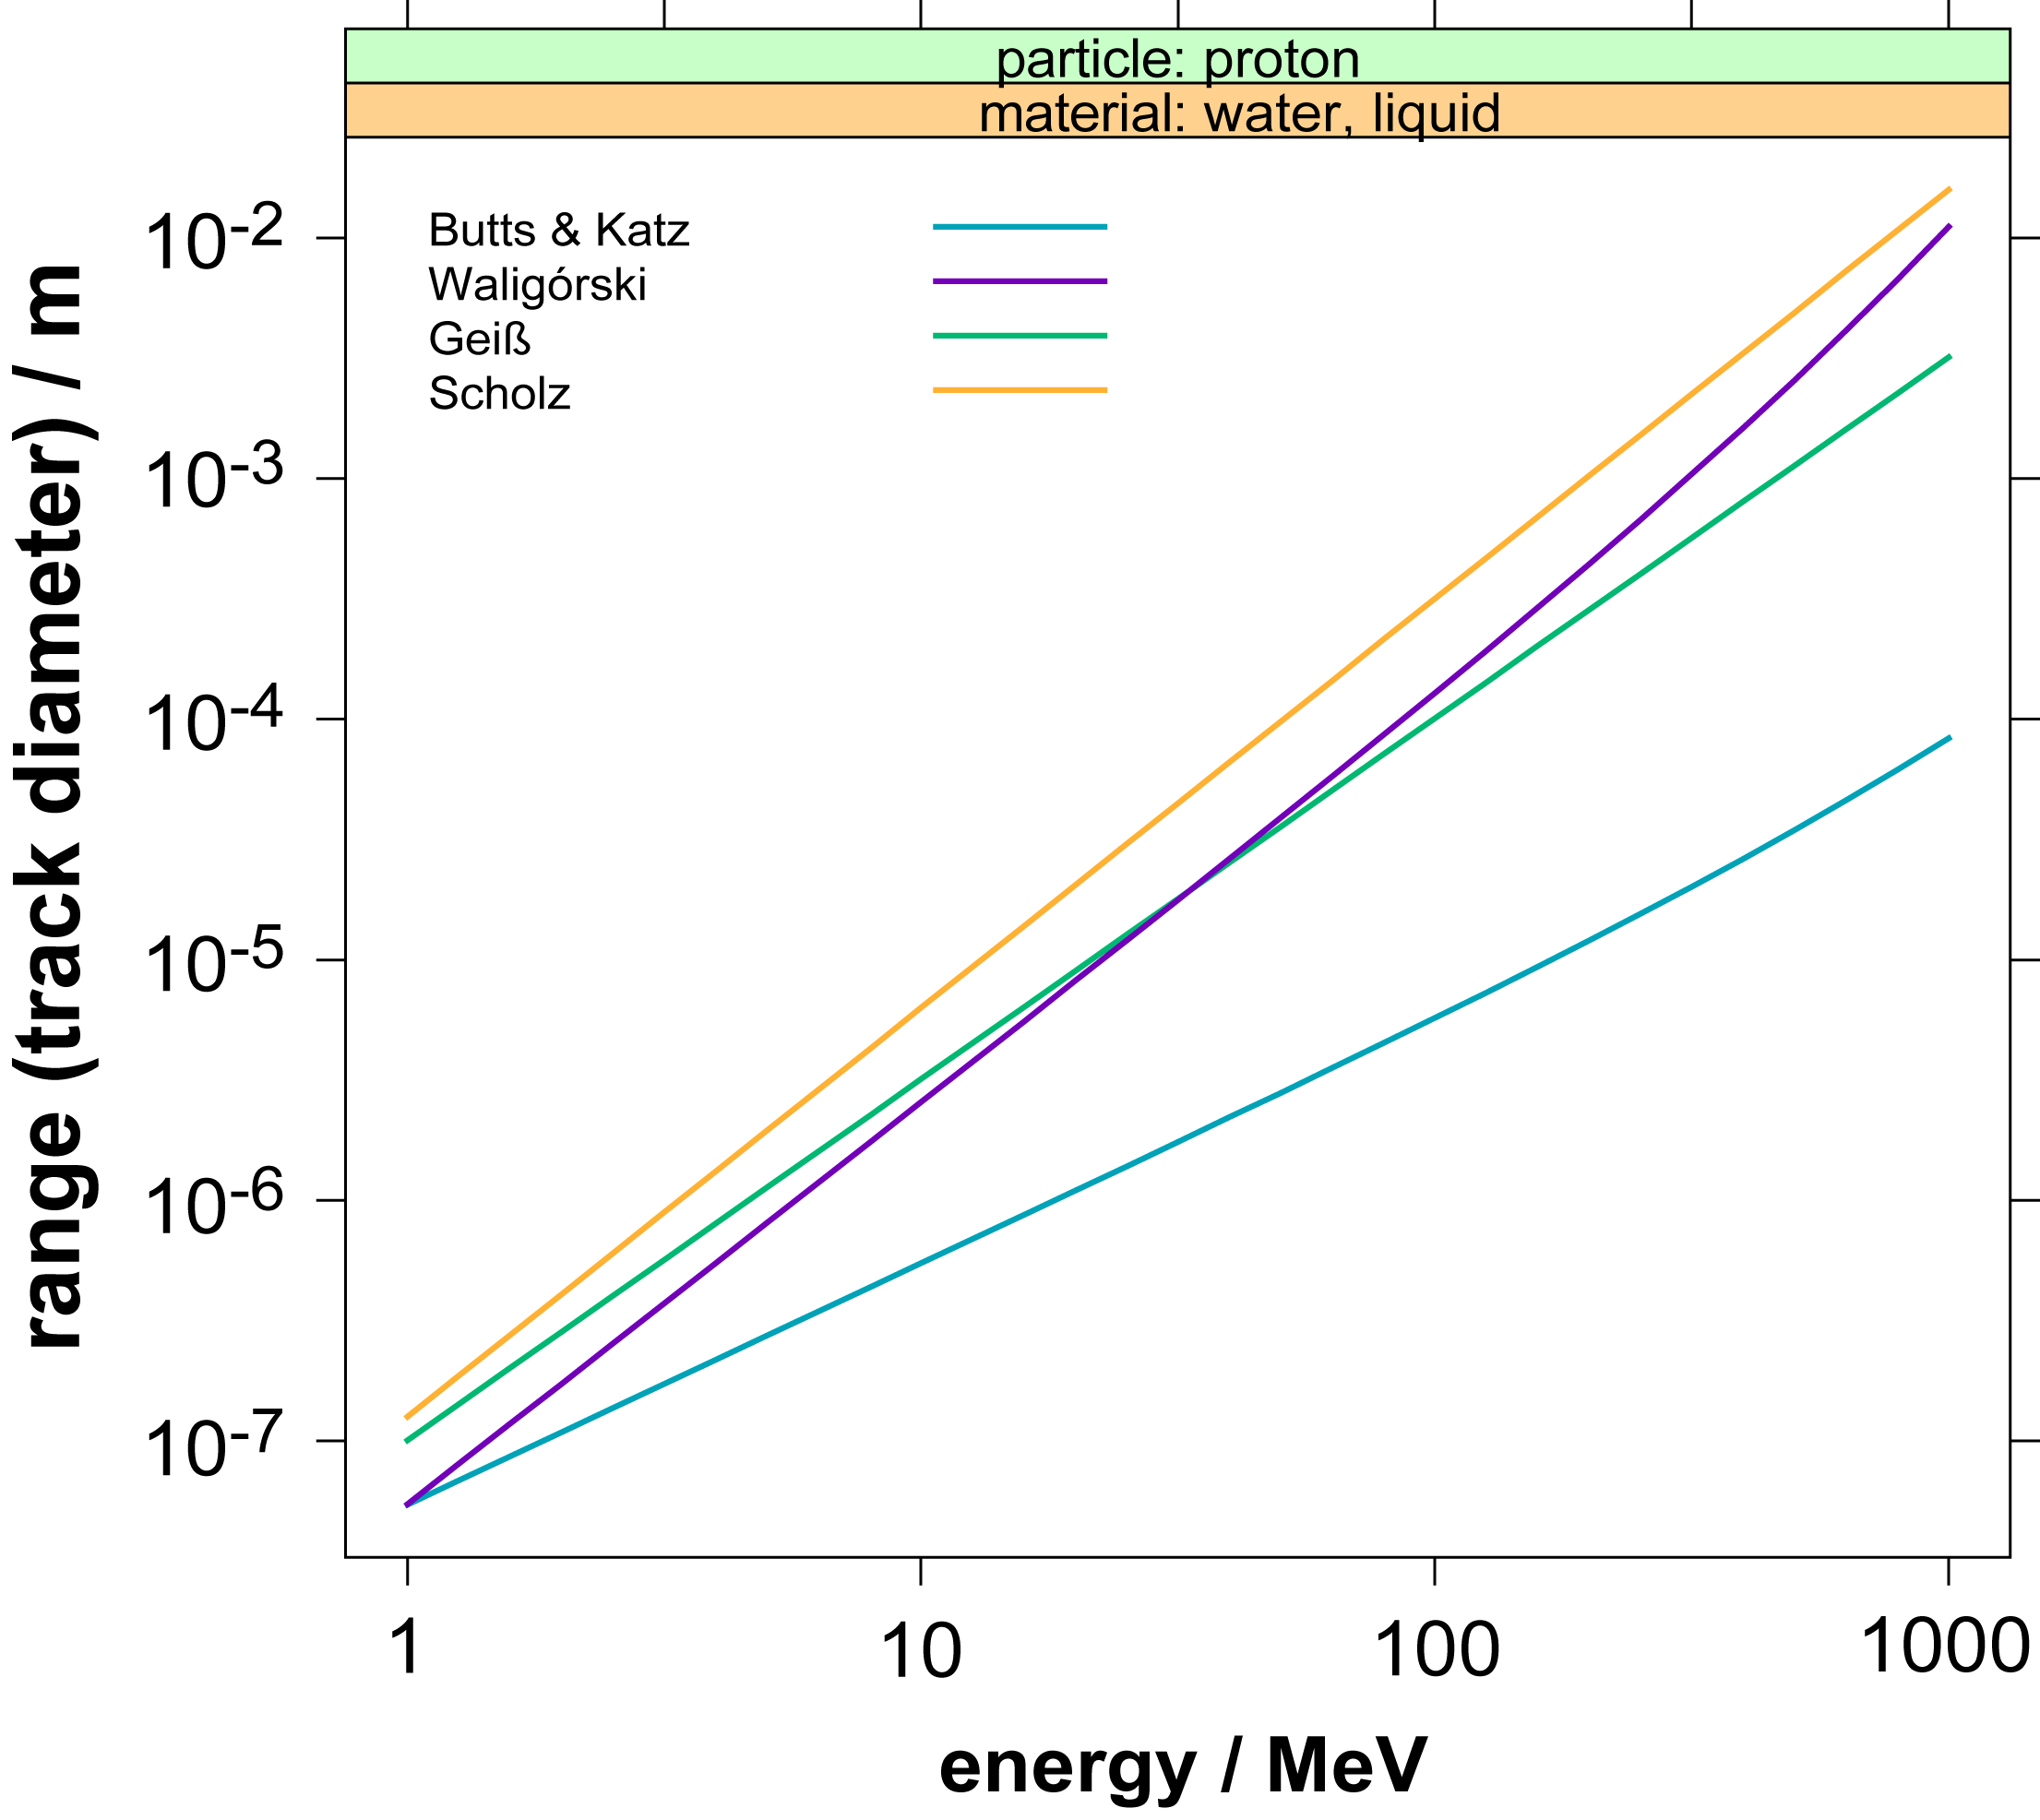
\includegraphics[width=1.0\textwidth]{pictures/ER.png}
	\caption{Electron-range submodels available in \la{}.}
	\label{fig:ERs}
\end{figure*}


\section*{Document status}
\begin{tabular}{l l}
2010.06.01&Created by S. Greilich
\end{tabular}